\documentclass[11pt,letterpaper,twocolumn]{article}


\usepackage[utf8]{inputenc}
\usepackage[spanish]{babel}
\usepackage{float}
\usepackage{xcolor}
\usepackage{verbatim}
\usepackage{charter}
\usepackage{amsmath}
\usepackage{appendix}
\usepackage{ragged2e}
\usepackage{array}
\usepackage{etoolbox}
\usepackage{fancyhdr}
\usepackage{booktabs}
\usepackage{arydshln}
\usepackage{caption}
\usepackage{subcaption}
\usepackage{enumitem}
\usepackage{geometry}
\geometry{
  top=0.8in,            
  inner=0.5in,
  outer=0.5in,
  bottom=0.9in,
  headheight=4ex,       
  headsep=6.5ex,         
}
\usepackage{graphicx}
\usepackage{mathtools}
\usepackage{multirow}
\usepackage{pdfpages}
\usepackage{subfiles}
\usepackage[compact]{titlesec}
\usepackage{stfloats}

\setlength{\columnsep}{30pt}


\pagestyle{fancy}
\fancyhf{}
      
\fancyfoot{}
\fancyfoot[C]{\thepage} % page
\renewcommand{\headrulewidth}{0mm} % headrule width
\renewcommand{\footrulewidth}{0mm} % footrule width

\makeatletter
\patchcmd{\headrule}{\hrule}{\color{black}\hrule}{}{} % headrule
\patchcmd{\footrule}{\hrule}{\color{black}\hrule}{}{} % footrule
\makeatother

\definecolor{blueM}{cmyk}{1.0,0.49,0.0,0.47}



\chead[C]{
      \begin{tabular}{m{1.5cm}m{11.5cm}m{2.5cm}}
      
\includegraphics[height=1.5cm]{imagenes/logo.png}
      &
      \centering
     \fcolorbox{white}{blueM}{\fbox{\begin{minipage}{11.5cm}
     \centering
     \textcolor{white}{ UNIVERSIDAD NACIONAL DE COLOMBIA}
     \end{minipage}}}
         &
        \centering
         \tiny{ \vspace{3.5mm} PROGRAMACIÓN EN LENGUAJES ESTADÍSTICOS\\
%%%%%%%%%%%%%%%%%%%%%%%%%%%%%%%%%%%%%%%%%%%%%%%%%%%%%%%%%%%%%%%%%%%%%%%%%%%%%%%%%%%%%%%%%%%%%%%%%
          Ciclo escolar: 2022-1\\ %Elija el ciclo que corresponda
%%%%%%%%%%%%%%%%%%%%%%%%%%%%%%%%%%%%%%%%%%%%%%%%%%%%%%%%%%%%%%%%%%%%%%%%%%%%%%%
          }\tabularnewline
%          \hline
          \end{tabular}%
    }
    
\begin{document}
\twocolumn[\begin{@twocolumnfalse}


\begin{minipage}{0.15\textwidth}{
    
\includegraphics[width=4cm]{imagenes/escudo.jpg}}
\end{minipage}
\hspace{25pt}
\begin{minipage}{0.75\textwidth}
\vspace{5mm}
    \Large{\textbf{Proyecto Estadísticas Cafeteras}} 
    \vspace{3mm}
    
    \large{\textbf{Autores:} Carrascal Deiver$^{1}$, Díaz Eduard$^{2}$,Guevara Eduardo$^{3}$, Mejia Bunkuaney$^{4}$}
    \vspace{2mm}
    
    \textbf{Docente 1:} Jose Francisco Ruiz Muñoz \newline
    
    \fontsize{0.35cm}{0.5cm}\selectfont \textit{Programación en Lenguajes estadísticos, Universidad Nacional de Colombia}
    \vspace{1mm} 
    
    \today % FECHA

\end{minipage}

\small

\vspace{11pt}

\centerline{\rule{0.95\textwidth}{0.4pt}}

\begin{center}
    
    \begin{minipage}{0.9\textwidth}
        % RESUMEN
        \noindent \textbf{Resumen:} Colombia es uno de los mayores productores de café del mundo,colombia junto con Brasil y Vietnam  representan 32,7 por ciento de las exportaciones mundiales de café, en el presente documento se encontrara un corto análisis estadístico de los datos proporcionados por la pagina oficial de la federación nacional de cafeteros.
    
        \vspace{4mm}
        % PALABRAS CLAVE
        \noindent \textbf{Palabras clave:} Café,Análisis, Exportaciones.
    
    \end{minipage}
     
    \begin{minipage}{0.9\textwidth}
        % abstract
         \vspace{4mm}
        \noindent \textbf{Abstract:} Colombia is one of the largest coffee producers in the world, Colombia together with Brazil and Vietnam represent 32.7 percent of world coffee exports, in this document you will find a brief statistical analysis of the data provided by the official page of the national federation of coffee growers.
    
        \vspace{4mm}
        % PALABRAS CLAVE
        \noindent \textbf{Keywords:} Coffee, Analysis, Exports.
    
    \end{minipage}
    
\end{center}

\centerline{\rule{0.95\textwidth}{0.4pt}}

\vspace{15pt}
\end{@twocolumnfalse}]
%%%%%%%%%%%%%%%%%%%%%%%%%%%%%%%%%%%%%%%%%%%%%%%%%%%%%%%%%%%%
\section{Introducción}
\justify
El café en Colombia, tiene alrededor de 300 años de historia, en el
año 1835 se exportaban los primeros sacos producidos en la zona
oriental, desde la aduana de cúcuta. Cuenta una leyenda que el
aumento de producción de café en Colombia fue gracias al sacerdote
jesuita Francisco Romero en un pueblo de Norte de Santander llamado
salazar de las palmas. El siguiente proyecto se basará en el
análisis estadístico (por medio de la programación) de este producto
tomando como referencia los datos que se encuentra en la página de la Federación Nacional de Cafeteros de Colombia, esto con el fin de poner en práctica lo aprendido en el módulo de Programación en lenguajes estadísticos y de igual forma aprender el papel que este producto ha estado desarrollando en la economía y en el desarrollo de este país. 
%%%%%%%%%%%%%%%%%%%%


\section{Marco Teórico}
\justify
La historia del café en Colombia gira en torno a historias y leyendas alrededor del este, datos históricos revelan que en 1730, los jesuitas trajeron el grano a la Nueva Granada, de la mano de viajeros provenientes de las Guayanas a través de Venezuela llegando a Colombia.\\
Uno de los más antiguos testimonios escritos, que se conoce acerca del cafeto en Colombia se le atribuye al sacerdote jesuita José Gumilla, quién en su libro El Orinoco Ilustrado (1730) registró la presencia del producto en la misión de Santa Teresa de Tabajé, llevada a cabo en cercanías a la desembocadura del río Meta en la Orinoquía.\\
Sin embargo ya para el año 1835, se registraron las primeras cosechas provenientes de la zona oriental del país, exportadas desde la aduana de Cúcuta. Esto en base a otra  leyenda, la cual hace referencia al sacerdote jesuita, Francisco Romero y sobre su papel en la expansión de este producto, ya que cuando los feligreses de la población de Salazar de las Palmas iban a congregarse, debían sembrar café por cada pecado que confesaban y así serían perdonados por Dios, acto que dió un gran impulso en la propagación del cultivo del grano.\\
Para la comprensión y análisis de todos los datos nos ayudaremos un lenguaje de programación llamado python el cual es un lenguaje
sencillo de leer y escribir debido a su alta similitud con el lenguaje humano. Así mismo se trata de un lenguaje multiplataforma de código abierto gratuito, lo que permite su desarrollo sin límites, además el uso de Python está muy extendido en dos áreas que han estado, y estarán, en boca de todos: el análisis de datos y el big data. Su simplicidad y su gran número de bibliotecas de procesamiento de datos hacen que Python sea ideal a la hora de analizar y gestionar una gran cantidad de datos en tiempo real.\\
Esto con el fin de llevar a cabo la solución de  los distintos ítem propuestos para la elaboración del proyecto, los cuales son:\\
\begin{enumerate}
    \item  precios,   área y producción del café.
    \item  exportaciones de café colombiano. Algunos de los análisis que se pueden incluir son:
    \begin{itemize}
        \item Gráficos de las variaciones de precio o producción a través del tiempo.
        \item Gráficas de precios estandarizados a precios de hoy (convirtiendo pesos de valor pasado a valor presente considerando la inflación).
        \item Pruebas estadísticas para comparar las medias de dos décadas (por ejemplo 1991-2000 vs 2001-2010) de los precios del café (utilizar precios estandarizados al valor presente).
        \item Diagramas de dispersión y correlaciones. Por ejemplo: Precio interno vs Volumen exportaciones.
        \end{itemize}
\end{enumerate}


%%%%%%%%%%%%%%%%%%%%%%%%%%%%%%%%%%%%%%%%%%%%%%%%%%%%%%%%%%%%
\section{Resultados y discusión}
\justify
\subsection{Gráficos de las variaciones de precio o producción a
través del tiempo}
Un gráfico de las variaciones del precio del café nos permitiría
analizar, como estos cambios afecta la compra y venta de este
producto.
 \begin{figure}[H]
            \centering
            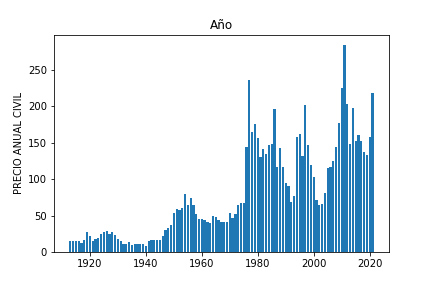
\includegraphics[width=0.5\textwidth]{imagenes/punto2_A.png}
            \caption{\label{fig1:frog}}
        \end{figure}
Un aumento o disminución de precios afecta a compradores,
competencia, distribuidores y proveedores; puede también llegar a
interesar al Gobierno y, por supuesto, a al gremio cafetero. 
Su éxito depende de cómo respondan las partes afectadas. 
Por eso uno de los puntos importantes a seguir en el comportamiento
en la economía atreves del tiempo y a partir de los datos que se
tienen se puedas seguir planteado bases de trabajo y la economía
cafetera sea un área productiva.\\

Por otra parte el precio del café en el año civil y en el año
cafetero tiene comportamiento similares, tenido crecimientos
importantes y algunos decaimientos durante el tiempo. No constante
se resalta que en las ultimas dos décadas este ha presentado las
elevaciones más significativas hasta la fecha, lo cual explica el
aumento exponencial en la producción y por consiguiente en los
consumidores, áreas de cultivo, empleos, entre otros factores en los
que se ve involucrado el campo café, como se denota en la siguiente
gráfica .
 \begin{figure}[H]
            \centering
            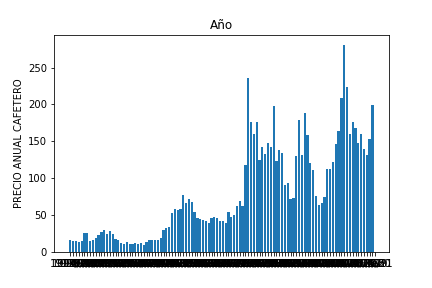
\includegraphics[width=0.5\textwidth]{imagenes/punto2_b.png}
            \caption{\label{fig2:frog}}
        \end{figure}
        


\subsection{Gráficas de precios estandarizados a precios de hoy (convirtiendo pesos de valor pasado a valor presente considerando la inflación).}
Las gráficas de los precios estandarizados nos permite hacer comparaciones directas entre la variaciones del precio del café através del tiempo, ya que permite ver como a afectado la inflación en el comportamiento de los  precios del café en el paso de los años.
\begin{figure}[H]
            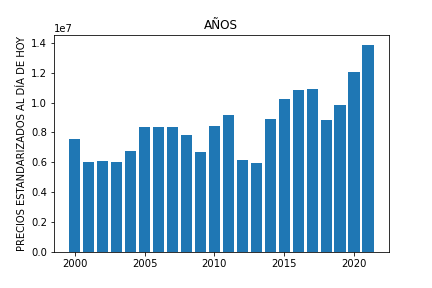
\includegraphics[width=0.5\textwidth]{imagenes/punto3.png}
            \caption{\label{fig3:frog}}
        \end{figure}
En la anterior gráfica podemos apreciar los precios estandarizados a precios de hoy, cuyos valores están  dados en miles de millones(e7), estos serian las ganancias anuales producidas por sector cafetero,  desde el año 2000 hasta el año 2021, teniendo en cuenta la inflación,los datos reales fueron tomados desde  la página oficial de la Federación Colombiana de Cafeteros, y posteriormente se estandarizo, en la gráfica se puede  apreciar que el precio ha estado variando a lo largo del tiempo, llegado a estar en los últimos años mal alto de lo normal divido a las alzas inesperadas de la inflación debido a la pandemia del covid-19.

\subsection{Pruebas estadísticas para comparar las medias de dos
décadas (por ejemplo 1991-2000 vs 2001-2010) de los precios del café
(utilizar precios estandarizados al valor presente).}

A continuación podremos apreciar una breve comparación entre los
promedios de los precios estandarizados del café en dos décadas
diferentes en donde podemos apreciar que en la década que contienen
los años del2011-2020 los precios sobrepasan a los de la década 
anterior, todo esto debido a la alta demanda y aceptación  que este
producto ha generado a lo largo de su consumo.
\begin{figure}[H]
            \centering
            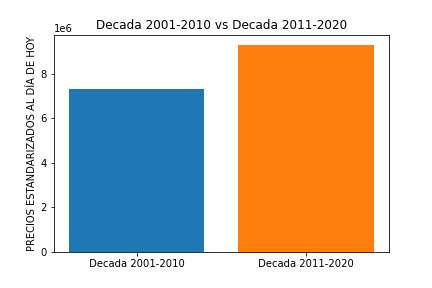
\includegraphics[width=0.5\textwidth]{imagenes/punto4.png}
            \caption{\label{fig4:frog}}
        \end{figure}
        
        
\subsection{Diagramas de dispersión y correlaciones. Por ejemplo: Precio interno vs Volumen exportaciones.}
Los diagramas de dispersión no mostraran la intensidad de la relación entre las  variables, en la figura 5 "El volumen total" vs año,  en la figura 6 "El volumen total" vs " El precio mensual",  y a demas la figura 7 es un diagrama de correlación de pearson el cual nos permite medir la relación estadística entre dos variables continuas.
\begin{figure}[H]
            \centering
            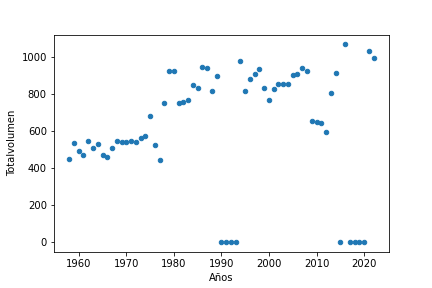
\includegraphics[width=0.5\textwidth]{imagenes/punto5_1.png}
            \caption{\label{fig5:frog}}
        \end{figure}
La gráfica 5 denota una leve tendencia, que se podría trazar mediante una línea unificadora, pero observamos que presenta valores atípicos por la parte de abajo, datos que afectan fuertemente la línea de tendencia y no permitirán una información pertinente.
\begin{figure}[H]
            \centering
            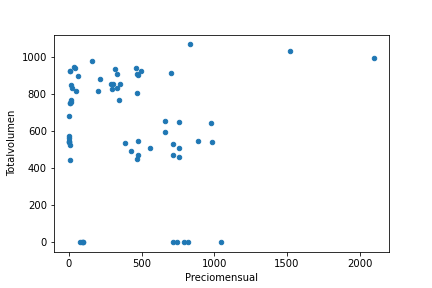
\includegraphics[width=0.5\textwidth]{imagenes/punto5_2.png}
            \caption{\label{fig6:frog}}
        \end{figure}
En la gráfica 6 Vemos cómo los datos están muy dispersos en la gráfica, no hay una tendencia clara por lo cual no se considera pertinente realizar la línea de tendencia ya que no tendría mucho sentido su resultado alejado de la mayoría de los datos.
\begin{figure}[H]
            \centering
            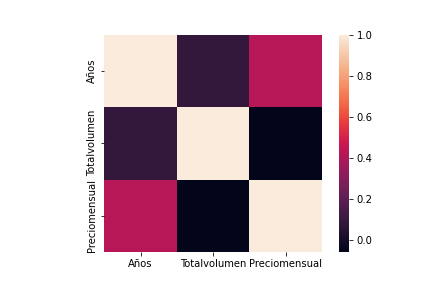
\includegraphics[width=0.5\textwidth]{imagenes/punto5_3.png}
            \caption{\label{fig7:frog}}
        \end{figure}
En la figura 7 como se menciono anteriormente es un diagrama de pearson, que en este caso cuneta en el eje x con tres variables distintas que son: año, volumen total y previo total, y el eje y cuenta con las mismas variables.\\
Lo que más nos importa es la relación entre  entre las variables traficadas,
El coeficiente de correlación de Pearson, para "Precio mensual" y "Año" es de aproximadamente 0.5,  por lo que podemos considerar que existe una relación entre ambas variables.

\section{Referencias}
\begin{itemize}
    \item HISTORIA DEL CAFÉ DE COLOMBIA. (2020, enero 21). Café de Colombia. https://www.cafedecolombia.com/particulares/historia-del-cafe-de-colombia/

    \item Díaz, S. (2020, octubre 20). Historia del café en Colombia. tienda-del-cafe-colombia. https://latiendadelcafe.co/blogs/cafe-colombiano/historia-del-cafe-en-colombia

    \item Estadísticas Cafeteras. (2019, noviembre 30). Federación Nacional de Cafeteros. https://federaciondecafeteros.org/wp/estadisticas-cafeteras/

    \item Python: qué es y por qué deberías aprender a utilizarlo. (s/f). Becas-santander.com. Recuperado el 2 de julio de 2022, de https://www.becas-santander.com/es/blog/python-que-es.html
\end{itemize}
  

\end{document}
